\documentclass[a4paper,11pt]{refart}

\usepackage[utf8]{inputenc}
\usepackage[T1]{fontenc} % LY1 also works

%% Font settings suggested by fbb documentation.
\usepackage{textcomp} % to get the right copyright, etc.
\usepackage[lining,tabular]{fbb} % so math uses tabular lining figures
\usepackage[scaled=.95,type1]{cabin} % sans serif in style of Gill Sans
\usepackage[varqu,varl]{zi4}% inconsolata typewriter
\useosf % change normal text to use proportional oldstyle figures
%\usetosf would provide tabular oldstyle figures in text

\usepackage{microtype}

\usepackage{graphicx}
\usepackage{enumitem}
\setlist{leftmargin=*}
\usepackage{listings}
\lstset{basicstyle=\ttfamily,frame=single,xleftmargin=3em,xrightmargin=3em}
\usepackage[os=win]{menukeys}
\renewmenumacro{\keys}[+]{shadowedroundedkeys}
\usepackage{framed}
\usepackage{etoolbox}
\AtBeginEnvironment{leftbar}{\sffamily\small}

\usetikzlibrary{chains,arrows,shapes,positioning}
\usepackage{hyperref}

\newcommand\AutoCalc{\textsf{AutoratingCalculator}}
\renewcommand\abstractname{Introduction}

\title{Autorating Calculator User Guide}
\author{Lim Lian Tze (\url{liantze@gmail.com})\\\url{http://liantze.penguinattack.org}}
\date{\url{https://bitbucket.org/liantze/autorating-calculator}\\July 13, 2013}
\begin{document}
\maketitle

\begin{abstract}
An `autorating' system uses peer ratings to award marks to individual students in team assignments \cite{Brown,KaufmanEtAl}. \AutoCalc{} is a simple tool intended to help educators streamline the calculation process of autorated marks, available for download at \url{https://bitbucket.org/liantze/autorating-calculator}. You will need a Java Runtime Environment ($\geq 1.6$)\footnote{\url{http://java.com/download}} to run it.
\end{abstract}

\tableofcontents
\clearpage

\section*{Quick Guide to Workflow}

%\begin{enumerate}
%\item 
%\end{enumerate}

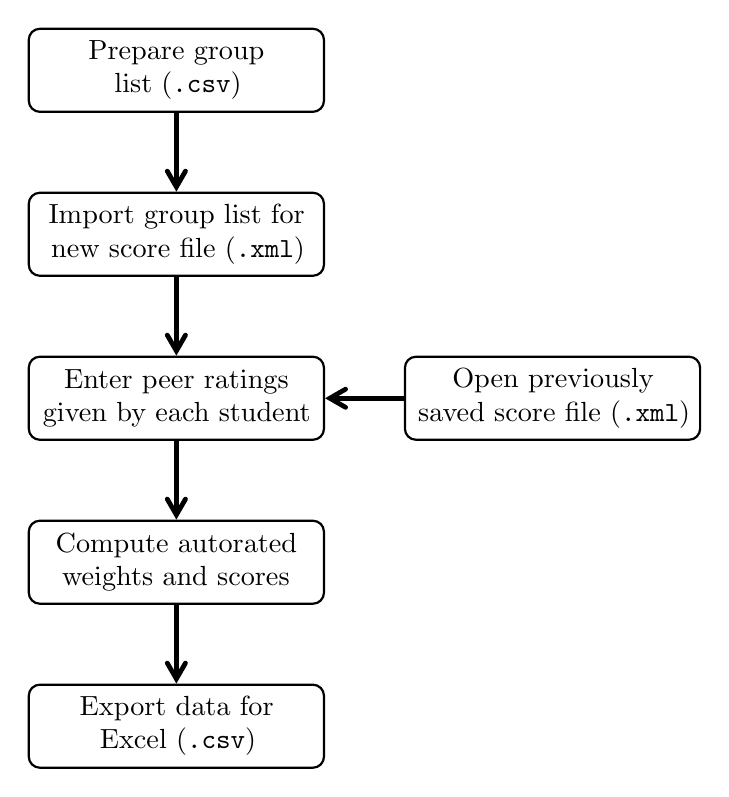
\begin{tikzpicture}
\tikzset{every node/.style={on chain,draw,thick,rounded corners,
minimum height=3em, text width=10em, align=center}}
\begin{scope}[start chain=going below]
\node (prepare-group) {Prepare group list (\texttt{.csv})};
\node (import-group) {Import group list for new score file (\texttt{.xml})};
\node (enter-rating) {Enter peer ratings given by each student};
\node (compute-score) {Compute autorated weights and scores};
\node (export-csv) {Export data for Excel (\texttt{.csv})};
\end{scope}
\node[right=of enter-rating] (open-score) {Open previously saved score file (\texttt{.xml})};

\path[draw,line width=0.4ex, ->,>= angle 60]
(prepare-group) edge (import-group) 
(import-group) edge (enter-rating)
(open-score) edge (enter-rating)
(enter-rating) edge (compute-score) 
(compute-score) edge (export-csv);
\end{tikzpicture}


\section{Preparing the Group List of a Class}

\begin{enumerate}
\item In Notepad, compile the list of group members in your class, using the following format:

\begin{lstlisting}
10032,Mary Tan
10143,Prabakar Murugan
10033,Tan Beng Huat
10165,Calvin Ong

10052,Mooi Siok Lan
10114,Bong Chin Keat
10432,Joseph Calvin
10281,Suresh Kappan
\end{lstlisting}

  \begin{itemize}[noitemsep]
  \item Record the \emph{ID} and \emph{name} of a student on each line.
  \item Use a comma (\texttt{,}) to separate the ID and name on each line.
  \item Leave an \emph{empty line} between groups.
  \end{itemize}
  
\item Save the group list file using \texttt{.txt} or \texttt{.csv} extension, e.g.\\\texttt{DIT1234-Apr2013-groups.txt}.

\medskip

\begin{leftbar}
You may also prepare the group list in Excel. List the IDs in column A and the IDs in column B. Save the file as a Comma separated values file (CSV). In the Export Filter Settings, set text delimiter to blank, and field separator to comma (\texttt{,}).
\end{leftbar}

\end{enumerate}

\section{Importing a Group List for a New Assignment Score File}

\begin{enumerate}
\item Launch the \AutoCalc\ tool by double-clicking on its icon in Windows Explorer.
\item From the menu bar, select \menu{File>Import...} or press \keys{Ctrl+I}.
\item Select a \emph{group list file} (\texttt{*.txt, *.csv}) to import from, e.g.\\\texttt{DIT1234-Apr2013-groups.txt}.
\item \AutoCalc\ will then ask you for a \emph{new} file name to save the new score list as (\texttt{*.xml}), e.g.~\texttt{DIT1234-Apr2013-Assgn1.xml}.


\medskip

\begin{leftbar}
Make sure the \texttt{.xml} score filename selected does not already exist. Otherwise the existing score file \textbf{may be overwritten without warning}!
\end{leftbar}

\medskip

\item \AutoCalc\ imports the group lists and displays the student IDs and names in the main panel (Figure~\ref{fig:grouplist}).

\begin{figure}[hbt!]\centering
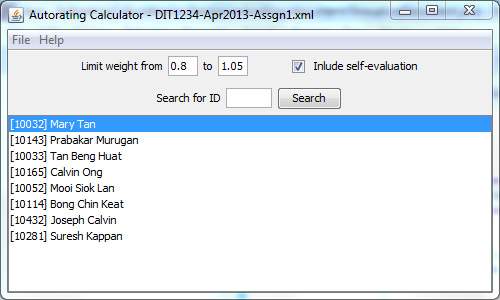
\includegraphics[width=\textwidth]{grouplist.png}
\caption{Imported group list}\label{fig:grouplist}
\end{figure}
\end{enumerate}

\section{Computing Autorated Scores from Group Scores and Peer Ratings}

\subsection{Setting Options}

Two options may be set at the top of the main \AutoCalc{} window.

\begin{itemize}
\item You may set the minimum and maximum autorating weight caps. Defaults are set at 0.8 and 1.02.

\item You may choose whether to include self-evaluated peer ratings. The default is to include self ratings.

\item If you change the settings, make sure to save them from the menu \menu{File>Save} or pressing \keys{Ctrl+S}.
\end{itemize}

\subsection{Selecting Students from List}

Double-click on the name of a student in the list to display the peer review score entry window.

\subsection{Searching Students by ID}

You can also load the peer ratings entry window of a student by keying in the ID number in the search box, and then click on the \keys{Search} button.

\subsection{Entering Scores and Ratings}

\begin{enumerate}
\begin{figure}[hbt!]
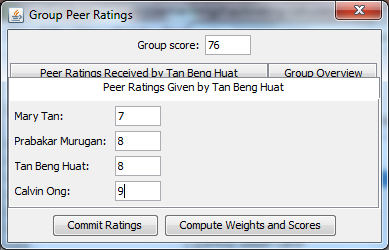
\includegraphics[width=\textwidth]{scorewindow.png}
\caption{Peer Ratings Window}
\end{figure}

\item In the peer ratings window for each student, enter the peer ratings given by the student to his/her teammates, including him/herself.
\item Enter also the overall score awarded to the group at the top of the window. (You only need to enter the group score once for each group.)
\item Click the  \keys{Commit Ratings} button to save the ratings.
\item Close the current peer rating window. Continue entering scores for other students.
\item You may click on the \keys{Peer Ratings Received by \ldots} tab to see ratings received by a student.

\begin{figure}[hbt!]
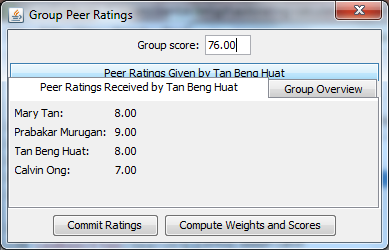
\includegraphics[width=\textwidth]{ratingsreceived.png}
\caption{Peer Ratings Received}
\end{figure}

\end{enumerate}

\subsection{Computing Autorated Scores}
\begin{enumerate}
\item When peer ratings of all students in a group has been entered and committed, click on the \keys{Compute Weights and Scores} button. The computed weights and scores will be saved to file immediately.
\item Click on the \keys{Group Overview} tab to see autorated weights and scores for each student in the group.

\begin{figure}[hbt!]
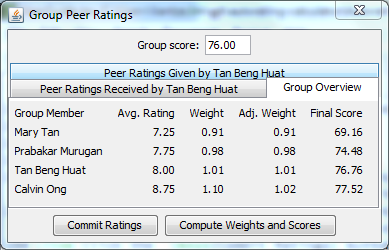
\includegraphics[width=\textwidth]{groupoverview.png}
\caption{Autorated Weights and Scores of Group Members}
\end{figure}

\end{enumerate}

\section{Opening Existing Assignment Score File}
You may open an existing assignment score file (\texttt{*.xml}) to inspect scores, as well as to change settings and recalculate scores.
\begin{enumerate}
\item To open an existing score file, access the menu item \menu{File>Open\ldots} or press \keys{Ctrl+O}.
\item Locate and select the \texttt{*.xml} file to open.
\end{enumerate}

\section{Exporting Data for Excel}
The autorated scores can be exported for further processing in Excel.
\begin{enumerate}
\item Select \menu{File>Export\ldots} from the menu, or \keys{Ctrl+E}.
\item Select a file name to save the exported data in. The file will be saved with a \texttt{.csv} extension. 
\includegraphics[height=1em]{csv.png}
\item In Windows Explorer, locate the \texttt{.csv} file and double-click on it to open it in Excel.
\item If warning messages are displayed, keep on clicking \keys{OK} or \keys{Yes} to ignore them.
\item When the data is displayed, you may save the file as an \texttt{.xlsx} or \texttt{.xsl} Excel file, and continue processing it.

\begin{figure}[hbt!]
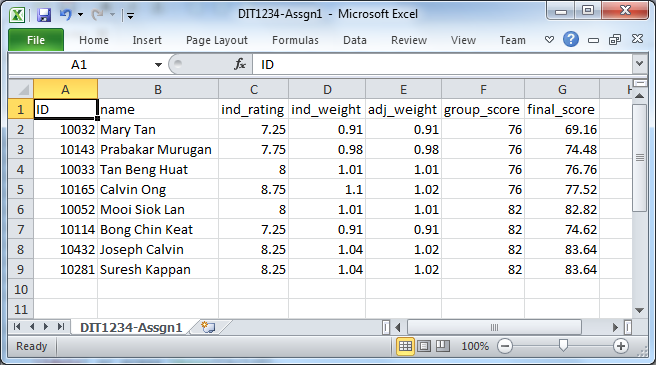
\includegraphics[width=\textwidth]{excel.png}
\caption{Exported data in Excel}
\end{figure}

\end{enumerate}

\bibliographystyle{plain}
\bibliography{refs}
\end{document}